\documentclass{article}

\usepackage{amssymb,amsmath,amsthm, enumerate, graphicx}
\graphicspath{{Pictures/}}
\usepackage{lipsum}
\usepackage{float} % Allows putting an [H] in \begin{figure} to specify the exact location of %the figure
\usepackage{wrapfig} % Allows in-line images such as the example fish picture
\usepackage[top=.20in]{geometry}
\usepackage[pdftitle = {Cal Poly CSC 305}, pdfauthor = {Matthew Jimenez}, pdfsubject = {Lab 06: Hollow Star}, colorlinks = true, urlcolor = blue]{hyperref}

\title{Lab 06 Design}
\author{Scott Rizzo}
\date{\today}

\begin{document}
\maketitle

\section{Class Diagram}
\begin{figure}[H]
\center{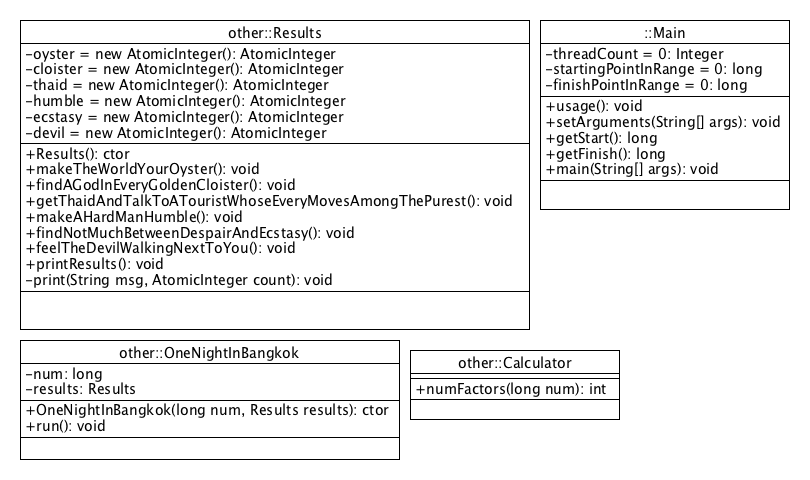
\includegraphics[width=0.8\linewidth]{lab07ClassDiagram}}
\caption{Class Diagram}
\label{fig:Hollow Star}
\end{figure}

\section{Class Responsibilities}
\subsection{Model}
The \texttt{model} is responsible for initializing the Circle objects in a data structure with there appropriate positions. It is a thread and will have multiple StarUI's associated with it and when it changes a random circle's color it notifies the StarComponents first then the StarUI's using the observer pattern to change.

\subsection{StarUI}
\texttt{StarUI} is responsible for adding the content of each each StarComponent to the screen. It also handles listening for when a screen is exited to invoke the appropriate methods.

\subsection{StarComponent}
The \texttt{StarComponent} is responsible for displaying and sizing each circle in its appropriate location based on where it's located in the data structure.

\subsection{Circle}
The \texttt{Circle} class is responsible holding the data associated with the circles position and color. It also has a method to convert into pixels but I could possible encapsulate that somewhere else.




\end{document}